\documentclass[]{article}
\usepackage{lmodern}
\usepackage{amssymb,amsmath}
\usepackage{ifxetex,ifluatex}
\usepackage{fixltx2e} % provides \textsubscript
\ifnum 0\ifxetex 1\fi\ifluatex 1\fi=0 % if pdftex
  \usepackage[T1]{fontenc}
  \usepackage[utf8]{inputenc}
\else % if luatex or xelatex
  \ifxetex
    \usepackage{mathspec}
  \else
    \usepackage{fontspec}
  \fi
  \defaultfontfeatures{Ligatures=TeX,Scale=MatchLowercase}
\fi
% use upquote if available, for straight quotes in verbatim environments
\IfFileExists{upquote.sty}{\usepackage{upquote}}{}
% use microtype if available
\IfFileExists{microtype.sty}{%
\usepackage{microtype}
\UseMicrotypeSet[protrusion]{basicmath} % disable protrusion for tt fonts
}{}
\usepackage[margin=1in]{geometry}
\usepackage{hyperref}
\hypersetup{unicode=true,
            pdftitle={Machine Learning for Optimal Stopping Problems with mlOSP},
            pdfauthor={Mike Ludkovski},
            pdfborder={0 0 0},
            breaklinks=true}
\urlstyle{same}  % don't use monospace font for urls
\usepackage{color}
\usepackage{fancyvrb}
\newcommand{\VerbBar}{|}
\newcommand{\VERB}{\Verb[commandchars=\\\{\}]}
\DefineVerbatimEnvironment{Highlighting}{Verbatim}{commandchars=\\\{\}}
% Add ',fontsize=\small' for more characters per line
\usepackage{framed}
\definecolor{shadecolor}{RGB}{248,248,248}
\newenvironment{Shaded}{\begin{snugshade}}{\end{snugshade}}
\newcommand{\KeywordTok}[1]{\textcolor[rgb]{0.13,0.29,0.53}{\textbf{#1}}}
\newcommand{\DataTypeTok}[1]{\textcolor[rgb]{0.13,0.29,0.53}{#1}}
\newcommand{\DecValTok}[1]{\textcolor[rgb]{0.00,0.00,0.81}{#1}}
\newcommand{\BaseNTok}[1]{\textcolor[rgb]{0.00,0.00,0.81}{#1}}
\newcommand{\FloatTok}[1]{\textcolor[rgb]{0.00,0.00,0.81}{#1}}
\newcommand{\ConstantTok}[1]{\textcolor[rgb]{0.00,0.00,0.00}{#1}}
\newcommand{\CharTok}[1]{\textcolor[rgb]{0.31,0.60,0.02}{#1}}
\newcommand{\SpecialCharTok}[1]{\textcolor[rgb]{0.00,0.00,0.00}{#1}}
\newcommand{\StringTok}[1]{\textcolor[rgb]{0.31,0.60,0.02}{#1}}
\newcommand{\VerbatimStringTok}[1]{\textcolor[rgb]{0.31,0.60,0.02}{#1}}
\newcommand{\SpecialStringTok}[1]{\textcolor[rgb]{0.31,0.60,0.02}{#1}}
\newcommand{\ImportTok}[1]{#1}
\newcommand{\CommentTok}[1]{\textcolor[rgb]{0.56,0.35,0.01}{\textit{#1}}}
\newcommand{\DocumentationTok}[1]{\textcolor[rgb]{0.56,0.35,0.01}{\textbf{\textit{#1}}}}
\newcommand{\AnnotationTok}[1]{\textcolor[rgb]{0.56,0.35,0.01}{\textbf{\textit{#1}}}}
\newcommand{\CommentVarTok}[1]{\textcolor[rgb]{0.56,0.35,0.01}{\textbf{\textit{#1}}}}
\newcommand{\OtherTok}[1]{\textcolor[rgb]{0.56,0.35,0.01}{#1}}
\newcommand{\FunctionTok}[1]{\textcolor[rgb]{0.00,0.00,0.00}{#1}}
\newcommand{\VariableTok}[1]{\textcolor[rgb]{0.00,0.00,0.00}{#1}}
\newcommand{\ControlFlowTok}[1]{\textcolor[rgb]{0.13,0.29,0.53}{\textbf{#1}}}
\newcommand{\OperatorTok}[1]{\textcolor[rgb]{0.81,0.36,0.00}{\textbf{#1}}}
\newcommand{\BuiltInTok}[1]{#1}
\newcommand{\ExtensionTok}[1]{#1}
\newcommand{\PreprocessorTok}[1]{\textcolor[rgb]{0.56,0.35,0.01}{\textit{#1}}}
\newcommand{\AttributeTok}[1]{\textcolor[rgb]{0.77,0.63,0.00}{#1}}
\newcommand{\RegionMarkerTok}[1]{#1}
\newcommand{\InformationTok}[1]{\textcolor[rgb]{0.56,0.35,0.01}{\textbf{\textit{#1}}}}
\newcommand{\WarningTok}[1]{\textcolor[rgb]{0.56,0.35,0.01}{\textbf{\textit{#1}}}}
\newcommand{\AlertTok}[1]{\textcolor[rgb]{0.94,0.16,0.16}{#1}}
\newcommand{\ErrorTok}[1]{\textcolor[rgb]{0.64,0.00,0.00}{\textbf{#1}}}
\newcommand{\NormalTok}[1]{#1}
\usepackage{graphicx,grffile}
\makeatletter
\def\maxwidth{\ifdim\Gin@nat@width>\linewidth\linewidth\else\Gin@nat@width\fi}
\def\maxheight{\ifdim\Gin@nat@height>\textheight\textheight\else\Gin@nat@height\fi}
\makeatother
% Scale images if necessary, so that they will not overflow the page
% margins by default, and it is still possible to overwrite the defaults
% using explicit options in \includegraphics[width, height, ...]{}
\setkeys{Gin}{width=\maxwidth,height=\maxheight,keepaspectratio}
\IfFileExists{parskip.sty}{%
\usepackage{parskip}
}{% else
\setlength{\parindent}{0pt}
\setlength{\parskip}{6pt plus 2pt minus 1pt}
}
\setlength{\emergencystretch}{3em}  % prevent overfull lines
\providecommand{\tightlist}{%
  \setlength{\itemsep}{0pt}\setlength{\parskip}{0pt}}
\setcounter{secnumdepth}{0}
% Redefines (sub)paragraphs to behave more like sections
\ifx\paragraph\undefined\else
\let\oldparagraph\paragraph
\renewcommand{\paragraph}[1]{\oldparagraph{#1}\mbox{}}
\fi
\ifx\subparagraph\undefined\else
\let\oldsubparagraph\subparagraph
\renewcommand{\subparagraph}[1]{\oldsubparagraph{#1}\mbox{}}
\fi

%%% Use protect on footnotes to avoid problems with footnotes in titles
\let\rmarkdownfootnote\footnote%
\def\footnote{\protect\rmarkdownfootnote}

%%% Change title format to be more compact
\usepackage{titling}

% Create subtitle command for use in maketitle
\newcommand{\subtitle}[1]{
  \posttitle{
    \begin{center}\large#1\end{center}
    }
}

\setlength{\droptitle}{-2em}
  \title{Machine Learning for Optimal Stopping Problems with mlOSP}
  \pretitle{\vspace{\droptitle}\centering\huge}
  \posttitle{\par}
  \author{Mike Ludkovski}
  \preauthor{\centering\large\emph}
  \postauthor{\par}
  \predate{\centering\large\emph}
  \postdate{\par}
  \date{April 16, 2018}


\begin{document}
\maketitle

{
\setcounter{tocdepth}{3}
\tableofcontents
}
\subsection{Simulation Based Optimal Stopping and
Beyond}\label{simulation-based-optimal-stopping-and-beyond}

Numerical resolution of optimal stopping problems has been an active
area of research for more than 2 decades. Originally investigated in the
context of American Option pricing, it has since metamorphosed into a
field unto itself, with numerous wide-ranging applications and dozens of
proposed approaches.

A major strand, which is increasingly dominating the subject, are
simulation-based methods that apply the Monte Carlo paradigm to Optimal
Stopping. With its roots in 1990s, this framework remains without an
agreed-upon name; we shall refer to it as Regression Monte Carlo (RMC).
The main feature of RMC is its marriage of a probabilistic approach,
namely direct reliance on the underlying stochastic state dynamics as
part of the simulations, and statistical tools for approximating the
quantities of interest, primarily the value and/or continuation
functions. This combination of simulation and statistics brings
scalability, flexibility in terms of underlying model assumptions and a
vast arsenal of potential implementations. These benefits have
translated into excellent performance which has made RMC popular both in
the academic and practitioner (quantitative finance) communities.
Indeed, in the opinion of the author, these developments can claim to be
the most successful numerical strategy that emerged from Financial
Mathematics. Dating back only about 20 years, they have now percolated
down into standard Masters-level curriculum, and are increasingly
utilized in cognate engineering and mathematical sciences domains.

Despite hundreds of journal publications addressing various variants of
RMC, there remains a dearth of user-friendly benchmarks or unified
overviews of the algorithms. In particular, to the author's knowledge,
there is no R (or other free programming languages such as Python)
package for RMC. One reason for this gap is the narrow focus of many
research articles that tend to explore one small aspect of RMC and then
illustrate their contributions on a small-scale, idiosyncratic example.

In the present article, I aim to offer an algorithmic template for RMC,
coupled with its implementation within R. This endevour is meant to be
an ongoing project, offering one way to centralize and standardize RMC
approaches, as they are proposed. In particular, the associated
\textbf{mlOSP} library is currently in its Version 1.0 incarnation, with
further (hopefully regular) updates to be fully expected.

\subsubsection{Contributions and
Outline}\label{contributions-and-outline}

This report offers a unified description of RMC via the underlying
statistical concepts. Hence, we describe a \emph{generic} RMC template
that emphasizes the building blocks, rather than specific approaches.
This perspective therefore aims to \emph{nest} as many of existing works
as possible, shedding light on the differences and the similarities
between the numerous proposals. To do so, we utilize as much as possible
the language of statistics (in contrast to the language of finance, or
of probability). In particular, we attempt to place RMC in the context
of modern machine/statistical learning, highlighting such aspects as
Design of Experiments, Simulation Device, and Sequential Learning.
Through this angle, we naturally connect RMC with numerous alternative
tools, twists, and extensions. Thus, we believe already the template is
an important contribution, giving a new take on some quite-old ideas.

Second, we propose several new variants based on the above templated
RMC. These include: * Adaptive kernel regression using nnreg and XXX and
svm * Varying the design size \(N\) across time-steps * hetGP/hetTP
regression * implementation of swing option via ML methods * sfjlksdjfl

Third, we introduce a few benchmarks, i.e.~fully specified problem
instances, that would be useful for other researchers.

The article is structured as an extended vignette and consists of two
parts. The first part lays out the RMC template which underlies the
\textbf{mlOSP} library. The template emphasizes the three pieces of RMC
framework: stochastic simulation, experimental design, and statistical
approximation. These pieces are modularized and can be fully
mixed-and-matched within the core backward dynamic programming loop
driving the algorithms. Section XXX briefly summarizes the variants of
each module that have been implemented, and includes references to the
original articles where these were proposed. For example, we provide
more than 10 different methods for the regression module, ranging from
kernel regression to piecewise linear regression to Gaussian process
regression.

The second part serves as a ``User Guide'' to mlOSP and illustrates how
the template is implemented in the library. For ease of use, we provide
about half-dozen top-level functions, whose usage is illustrated via
code listings and the respective R output. The latter is organized as a
RMarkdown document, enabling full reproduction by any reader who
downlaods the \textbf{mlOSP} package. Simultaneously with illustrating
\emph{how} to use \textbf{mlOSP}, we also define several instances of
OSP, including examples of Bermudan options in 1-, 2-, 3-, and
5-dimensions. By providing fully reproducible results on these
instances, we hope to create a preliminary set of simple benchmarks that
allow for a transparent, apples-to-apples comparison of different
methods. As we discuss below, the numerous nuances that inevitably crop
up when implementing RMC, frequently make such comparisons fraught,
leading to a lack of consensus on what strategies are more efficient.

The \textbf{mlOSP} library is meant to be extensible in the sense of
offering a simple interface to define new OSP instances. This is
achieved by utilizing, where possible, function pointers. For example, R
already offers a standardized interface for regression, consisting of
the \emph{fit} and \emph{predict} methods. \textbf{mlOSP} can then
piggy-back on that interface, allowing the user to easily ``hook-up'' a
new regression method for the regression module. Similarly,
\textbf{mlOSP} can easily handle user-defined system dynamics,
incorporated through constructing a new instance of path-simulator.
These features of \textbf{mlOSP} are illustrated at the end of the
``User Guide'' where we take examples from a couple of very recent
papers and show how they can be embedded into the \textbf{mlOSP}
template to facilitate comparison with existing ideas.

\subsection{Optimal Stopping and RMC}\label{optimal-stopping-and-rmc}

An optimal stopping problem is described through two main ingredients:
the state process and the reward function. We shall use \(X\) to denote
the state process, assumed to be a stochastic process indexed
generically by the time index \(t\). The reward function is \(h(t,x)\)
where the notation emphasizes the common possibility of the reward
depending on time, e.g.~due to discounting.

We seek the rule \(\tau\), a \emph{stopping time} to maximize expected
reward: \[\mathbb{E}[ h(\tau,X_\tau) ] \rightarrow \max! \] To this end,
we wish to evaluate the value function
\[V(t,x) = \sup_{\tau \in \cal{S}} \mathbb{E}[ h(\tau, X_\tau) | X_t = x ]\]

The state \((X_t)\) is typically assumed to satisfy a Stochastic
Differential Equation of Ito type,
\[  dX_t = \mu(X_t) \, dt + \sigma(X_t)\, dW_t,\] where \((W_t)\) is a
(multi-dimensional) Brownian motion.

To understand optimal stopping, it is most intuitive to think of it as a
dynamic decision making. At each exercise step, the controller must
decide whether to stop (0) or continue (1), which within a Markovian
structure is encoded via the action map \(A_t(x) \in \{ 0,1 \}\). This
action map gives rise to the stopping region
\[ {\cal S}_t = \{ x : A_t(x) = 0\} \] where the decision is to stop and
in parallel defines the corresponding
\(\tau = \min \{ t: A(X_t) = 0 \}\) Hence, solving an OSP is equivalent
to classifying each \(x\) into \({\cal S}_t\) or its complement the
continuation set. The respective objective function is the expected
reward:
\[ \widehat{V}(t,x)[A] := \mathbb{E}[ h(\tau_A, X^x_{\tau_A})].\]

The RMC construction relies on recursively constructing \(A_t\) based on
\((A_s : s > t)\). This is achieved by rephrasing
\[ A_t(x) = 1 \quad \Leftrightarrow \quad \mathbb{E}[ h(\tau_{A_{t+1}}, X^x_{\tau_{A_{t+1}}})] > h(t,x) \],
i.e.~one should contain if the expected reward-to-go dominates the
immediate payoff. The Dynamic Programming Principle implies that the
right-hand-side can be expressed as the conditional expectation of
\(V(t+1, X^x_{t+1})\), henceforth termed the continuation value
\[ q(t,x) = \mathbb{E}[ V(t+1, X^x_{t+1}) | X_t =x]. \]

This construction yields the following loop: 1. Set \(V(T,x)=h(T,x)\) 2.
For \(t=T-1,...,1\) i) Learn the conditional expectation
\(\hat{q}(t,\cdot) = \hat{E}[ \hat{V}(t+1, \cdot) | X_t = x]\) ii) Set
\(\hat{A}_t(x) = \{ 1 : \hat{q}(t,x) > h(t,x) \}\) iii) Set
\(\hat{V}(t,x) = \max ( \hat{q}(t,x), h(t,x))\) 3. Run out-of-sample
\[ \hat{V}(0,x_0) = \frac{1}{N'} \sum_{n'=1}^{N'} h(\tau_{\hat{A}(0)}, X_\tau)\]

The key step requiring numeric approximation is 2i. In the RMC paradigm
it is handled by re-interpreting conditional expectation as the mean
response within a stochastic input-output model. Thus, given an input
\(x\), there is a generative model which is not directly known but
accessible through a pathwise reward simulator. The aim is then to
predict the mean output of this simulator for an arbitrary \(x\).
Practically, this is done by running some simulations and then utilizing
a statistical model to capture the observed input-output relationship.
This statistical learning task can be broken further down into three
sub-problems: 1. Defining the stochastic simulator 2. Defining the
simulation design 3. Defining the regression step Recasting in the
machine learning terminology, we need to define a simulator that accept
a value \(x\) (the initial state at time \(t\)) and return \(Y\) which
is a random realization of the pathwise reward starting at \((t,x)\). We
then need to decide which collection of \(x\)'s should be applied as a
training set. After selecting such experimental design of size \(N\),
\(x^{1:N}\), we collect the \(y^{1:N} = Y(x^{1:N})\) and reconstruct the
model
\[ Y(x) = f(x) + \epsilon(x), \qquad \mathbb{E}[ \epsilon(x)] = 0, \mathbb{Var}(\epsilon(x)) = \sigma^2(x)\]
where \(f(x) \equiv \hat{q}(t,x)\).

We now make a few remarks: * The procedure is recursive, necessarily the
simulator at step \(t\) is linked to the previous simulators at steps
\(s > t\). Therefore, errors will tend to back-propagate. * There is no
``data'' per se, the controller is fully in charge of selecting what
simulations to run. Judicious choice of how to do so is our primary
criterion of numerical efficiency. Deciding how to train \(\hat{q}\) is
a key step in RMC. * In classical ML tasks, there is a well-defined loss
functions that quantifies the quality of the constructed approximation.
In OSP, this loss function is highly implicit; ultimately we judge
algorithm performance in terms of the final \(\hat{V}(0,x_0)\) (higher
is better). Thus, one must construct heuristics to translate this into
the loss function for the local learning task. * RMC is a
\textbf{sequence} of tasks, indexed by \(t\). While the tasks are
inter-related, since they are solved one-by-one, there is a large scope
for modularization, adaptation, etc to be utilized. * The stochasticity
in RMC comes from using the pathwise simulator and is ultimately based
on the random shocks driving the evolution of \((X_t)\). Thus, the
stochasticity is deeply imbedded in the problem. Because it is so
intrinsic, \(\epsilon(x)\) must be understood not as observation noise
but rather simulation noise. In particular, its statistical properties
tend to be quite complex and non-Gaussian. * The basic loop makes it
clear that like in standard regression, there ought to be a training set
(used in the backward iteration) and a test set, used for estimating
\(\hat{V}(0,x_0)\). Because the latter is essentially a plain MC
estimate of expected reward given the specific stopping rule
\(\tau(\hat{A})\), ie. of
\(\mathbb{E}[ h(\tau_{\hat{A}(0)}, X_{\tau_{\hat{A}(0)}})]\), modulo MC
error (captured by the LLN and CLT) it will yield a lower bound on the
true maximum expected reward. In contrast, any attempt to use the
training data to estimate expected rewards cannot come with any
reasonably upper/lower bound guarantees.

\subsubsection{Dynamic Emulation
Template}\label{dynamic-emulation-template}

Put the algorithm in here

\subsubsection{Bringing it Back into Focus: Bermudan Option
Pricing}\label{bringing-it-back-into-focus-bermudan-option-pricing}

To offer the most intuitive context for using \textbf{mlOSP}, the
vignette below focuses on OSP instances coming from Bermudan option
pricing. In this context, we take the point of view of a buyer of an
American option, which is a financial contract that gives the holder the
ability (but not the obligation) to obtain a certain payoff, contingent
on the underlying asset price. For example, an American Put allows its
owner the right to exchange the asset for a pre-specified strike \(K\),
equivalent to the payoff \((K-x)_+\). The contract has an expiration
date \(T\), and the exercise frequency is taken to be \(\Delta t\) (such
as daily). The state \(X_t\) is then interpreted as the
\emph{share price} of the asset at date \(t\), which is naturally must
be non-negative. Taking into account the time-value of money, it follows
that the reward function is \[
  h_{Put}(t,x) = e^{-r t} (K-x)_+,
\] where \(r\) is the constant interest rate.

With this setup, the stopping set is known as the exercise region.
Another term is the timing value, \(T(t,x) = q(t,x) - h(t,x)\), so that
exercising is optimal when the timing value is negative. The fact that
the reward has a lower bound of zero, reflects the optionality and the
fact that the holder can never lose money. It implies that
\(\epsilon(x)\) has a mixed distribution with a point mass of
zero\ldots{}

For Bermudan option pricing, the seminal breakthrough were the works of
Longstaff and Schwartz and Tsitsiklis and van Roy, that popularized the
RMC approach in this context. Especially the former, which contained a
simple toy example with \(N=8\) paths has been adopted as pedagogical
device to explain RMC. The LS approach proposed to use a single set of
global simulations, and to adopt the full pathwise simulator. Its other
insight was that due to the special structure, learning \(\hat{q}\) is
only necessary in-the-money, i.e.~in the region where \(h(t,x) >0\);
otherwise it is clear that \(T(t,x) > 0\) and hence \(A_t(x) = 1\).

Numerous methods have since embellished and improved LS. One
particularly large strand of literature has addressed different
regression variants: * Piecewise regression with adaptive sub-grids by
Bouchard and Warin * Regularized regression, such as LASSO, by Kohler
{]}Kohler and Krzyżak (2012){]} * Kernel regressoin by Belomestny et al
* Gaussian Process regression by Ludkovski * Neural nets by Kohler and
XXX * dynamic trees by Gramacy and Ludkovski (Gramacy and Ludkovski
2015)

\section{Getting Started with mlOSP}\label{getting-started-with-mlosp}

The following user guide highlights the key aspects of mlOSP. It is
intended to be fully reproducible, so that the reader can simply
cut-and-paste (or download the RMarkdown document online) the R code.
Since all the algorithms are intrinsically based on generating random
outputs based on the underlying stochastic simulator, where possible we
fix the RNG seeds. Depending on the particular machine and R version,
the seeds might nevertheless lead to different results.

Load the necessary libraries (there are quite a few since we try many
different regression methods)!

\begin{Shaded}
\begin{Highlighting}[]
\KeywordTok{library}\NormalTok{(ks)}
\KeywordTok{library}\NormalTok{(fields) }\CommentTok{# for plotting purposes, use quilt.plot in 2D}
\KeywordTok{library}\NormalTok{(seqOSP)}
\KeywordTok{library}\NormalTok{(DiceKriging)}
\KeywordTok{library}\NormalTok{(tgp)  }\CommentTok{# use lhs from there}
\KeywordTok{library}\NormalTok{(randtoolbox)  }\CommentTok{# use sobol and halton QMC sequences}
\KeywordTok{library}\NormalTok{(randomForest)}
\KeywordTok{library}\NormalTok{(earth)}
\KeywordTok{library}\NormalTok{(hetGP)}
\KeywordTok{library}\NormalTok{(kernlab)}
\end{Highlighting}
\end{Shaded}

The seqOSP library has several principal schemes for constructing the
emulators that describe the estimated stopping rule. The emulators are
indexed by the underlying type of simulation \emph{design} which most
affects the implementation. We have:

\begin{itemize}
\item
  osp.prob.design -- this is the original Longstaff Schwartz scheme that
  generates forward trajectories that are then re-used as the design
  sites. In our notation, this is a pure probabilistic design, without
  any replication. It is married to a variety of regression methods,
  both parametric and nonparametric.
\item
  osp.fixed.design -- the generic RMC scheme with a pre-specified/fixed
  (in the sense of not sequential) design. In particular the design can
  be replicated using \emph{km.batch} parameter. This approach nests the
  osp.prob.design when km.batch=1 and the input.domain is fully
  specified.
\item
  osp.probDesign.piecewisebw -- this is the Bouchard Warin
  implementation of RMC that utilizes a hierarchical (piecewise) linear
  model based on an equi-probable partition of the forward trajectory
  sites. Since we have a ``quick-and-dirty'' recursive construction of
  the sub-domains, the fits from this function \emph{cannot} be fed into
  a forward simulator. However, the function directly accepts a
  collection of test trajectories that are evaluated in parallel with
  the backward DP iteration.
\item
  mc.put.adaptree -- sequential RMC with \emph{dynaTree} emulators
\item
  osp.seq.design --- sequential RMC with GP (ie Stochastic Kriging)
  emulators that are used to construct sequential design acquisition
  functions via the posterior emulator variance
\end{itemize}

\subsubsection{1D Toy Example}\label{d-toy-example}

We start with a simple 1-D Bermudan Put. The underlying dynamics are
given by Geometric Brownian Motion
\[ dX_t = rX_t dt + \sigma X_t dW_t, \qquad X_0 = x_0\] In the model
specification below we have \(r=0.06, T=1, \sigma=0.2\) and the option
payoff is a Put \((K-X_t)_+\) with \(K=40\). The exercise is possible 25
times before expiration, i.e \(\Delta t = 0.04\).

We hand-build a few designs that cover the in-the-money region
\([25,40]\) using QMC sequences. As a start we use a Gaussian Process
emulator with a replicated design. The replications are treated using
the SK method (Ankenman et al 2012), pre-averaging the replicated
outputs before training the GP. The GP has a constant prior mean,
learned via the Universal Kriging equations (Ginsbourger et al 2013)

\begin{Shaded}
\begin{Highlighting}[]
\CommentTok{# a few prespecified designs}
\NormalTok{grid1 <-}\StringTok{ }\KeywordTok{c}\NormalTok{(}\DecValTok{30}\NormalTok{, }\DecValTok{33}\OperatorTok{:}\DecValTok{39}\NormalTok{)}
\NormalTok{grid2 <-}\StringTok{ }\KeywordTok{c}\NormalTok{(}\DecValTok{28}\NormalTok{, }\DecValTok{30}\NormalTok{, }\KeywordTok{seq}\NormalTok{(}\FloatTok{32.5}\NormalTok{, }\DecValTok{39}\NormalTok{, }\DataTypeTok{by=}\FloatTok{0.5}\NormalTok{))}
\NormalTok{grid3 <-}\StringTok{ }\KeywordTok{sort}\NormalTok{(}\DecValTok{15}\OperatorTok{*}\KeywordTok{sobol}\NormalTok{(}\DecValTok{15}\NormalTok{)}\OperatorTok{+}\DecValTok{25}\NormalTok{)}
\NormalTok{grid4 <-}\StringTok{ }\KeywordTok{sort}\NormalTok{(}\DecValTok{15}\OperatorTok{*}\KeywordTok{sobol}\NormalTok{(}\DecValTok{200}\NormalTok{)}\OperatorTok{+}\DecValTok{25}\NormalTok{)}

\CommentTok{# specify the simulation model, the payoff, and the emulator setup}
\NormalTok{model1 <-}\StringTok{ }\KeywordTok{c}\NormalTok{(}\DataTypeTok{final.runs=}\DecValTok{0}\NormalTok{, }\DataTypeTok{K=}\DecValTok{40}\NormalTok{,}\DataTypeTok{x0=}\DecValTok{40}\NormalTok{,}\DataTypeTok{sigma=}\FloatTok{0.2}\NormalTok{,}\DataTypeTok{r=}\FloatTok{0.06}\NormalTok{,}\DataTypeTok{div=}\DecValTok{0}\NormalTok{,}\DataTypeTok{T=}\DecValTok{1}\NormalTok{,}\DataTypeTok{dt=}\FloatTok{0.04}\NormalTok{,}\DataTypeTok{dim=}\DecValTok{1}\NormalTok{,}\DataTypeTok{sim.func=}\NormalTok{sim.gbm,}
 \DataTypeTok{lhs.rect=}\KeywordTok{c}\NormalTok{(}\DecValTok{25}\NormalTok{,}\DecValTok{40}\NormalTok{),}\DataTypeTok{init.size=}\DecValTok{15}\NormalTok{,}\DataTypeTok{km.cov=}\DecValTok{4}\NormalTok{,}\DataTypeTok{km.var=}\DecValTok{1}\NormalTok{,}\DataTypeTok{cand.len=}\DecValTok{1000}\NormalTok{,}\DataTypeTok{look.ahead=}\DecValTok{1}\NormalTok{)}

\NormalTok{put1d.model <-}\StringTok{ }\NormalTok{model1}
\NormalTok{put1d.model}\OperatorTok{$}\NormalTok{km.batch <-}\StringTok{ }\DecValTok{200}
\NormalTok{put1d.model}\OperatorTok{$}\NormalTok{pilot.nsims =}\StringTok{ }\DecValTok{0}
\NormalTok{put1d.model}\OperatorTok{$}\NormalTok{covfamily=}\StringTok{"matern5_2"}
\NormalTok{put1d.model}\OperatorTok{$}\NormalTok{N <-}\StringTok{ }\DecValTok{500}
\NormalTok{option.payoff <-}\StringTok{ }\NormalTok{put.payoff}

\CommentTok{# use the DiceKriging Gaussian Process emulator with fixed hyperparameters specified in}
\CommentTok{# km.cov, km.var. The default kernel is Matern-5/2}
\NormalTok{km.fit <-}\StringTok{ }\KeywordTok{osp.fixed.design}\NormalTok{(put1d.model,}\DataTypeTok{input.domain=}\NormalTok{grid3, }\DataTypeTok{method=}\StringTok{"km"}\NormalTok{)}
\end{Highlighting}
\end{Shaded}

Now we visualize the results from one time-step. To do so, we first
predict the timing value based on a fitted emulator (at \(t=10\Delta t\)
step) over a collection of points. We then plot the point estimate of
\(T(t,x)\) and the corresponding credible interval (which is organically
provided by the GP emulator).

\begin{Shaded}
\begin{Highlighting}[]
\NormalTok{check.x <-}\StringTok{ }\KeywordTok{seq}\NormalTok{(}\DecValTok{24}\NormalTok{, }\DecValTok{40}\NormalTok{, }\DataTypeTok{len=}\DecValTok{500}\NormalTok{)   }\CommentTok{# predictive sites}
\NormalTok{myCol <-}\StringTok{ "grey"}
\NormalTok{km.pred <-}\StringTok{ }\KeywordTok{predict}\NormalTok{(km.fit}\OperatorTok{$}\NormalTok{fit[[}\DecValTok{10}\NormalTok{]],}\KeywordTok{data.frame}\NormalTok{(}\DataTypeTok{x=}\NormalTok{check.x), }\DataTypeTok{type=}\StringTok{"UK"}\NormalTok{)  }\CommentTok{# syntax specific to km}
\KeywordTok{plot}\NormalTok{(check.x, km.pred}\OperatorTok{$}\NormalTok{mean, }\DataTypeTok{lwd=}\DecValTok{2}\NormalTok{, }\DataTypeTok{type=}\StringTok{"l"}\NormalTok{, }\DataTypeTok{xlim=}\KeywordTok{c}\NormalTok{(}\DecValTok{27}\NormalTok{,}\DecValTok{40}\NormalTok{), }\DataTypeTok{ylim=}\KeywordTok{c}\NormalTok{(}\OperatorTok{-}\FloatTok{0.4}\NormalTok{,}\FloatTok{1.1}\NormalTok{), }\DataTypeTok{xlab=}\StringTok{'X'}\NormalTok{, }\DataTypeTok{ylab=}\StringTok{'Timing Value'}\NormalTok{)}
\KeywordTok{lines}\NormalTok{(check.x, km.pred}\OperatorTok{$}\NormalTok{lower95, }\DataTypeTok{lty=}\DecValTok{2}\NormalTok{,}\DataTypeTok{col=}\NormalTok{myCol)  }\CommentTok{# 95% CI band, see documentation of predict.km}
\KeywordTok{lines}\NormalTok{(check.x, km.pred}\OperatorTok{$}\NormalTok{upper95, }\DataTypeTok{lty=}\DecValTok{2}\NormalTok{,}\DataTypeTok{col=}\NormalTok{myCol)}
\KeywordTok{abline}\NormalTok{(}\DataTypeTok{h=}\DecValTok{0}\NormalTok{,}\DataTypeTok{lty=}\DecValTok{2}\NormalTok{)}
\KeywordTok{rug}\NormalTok{(grid3, }\DataTypeTok{quiet=}\OtherTok{TRUE}\NormalTok{)}
\end{Highlighting}
\end{Shaded}

\begin{figure}
\centering
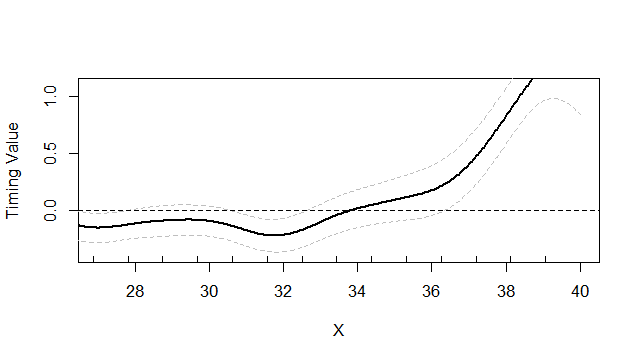
\includegraphics{figures/Fitted-GP-1.png}
\caption{Timing Value of a Bermudan Put based on GP emulator. We also
display the underlying simulation design (the rug plot) and the
uncertainty quantification regarding the fit of T(t,x) (the shaded 95
CI)}
\end{figure}

\subsubsection{2D Average Put example}\label{d-average-put-example}

Next we try a 2D example where things get a bit more interesting. Here
the payoff is the basket average Put, \[ (K - (X_1+X_2)/2)_+\]. We
continue to use \(K=40\). Thus, the option is in-the-money when
\(X_1+X_2 > 80\) in the example below. For the initial condition we
primarily use \((40,40)\) which is At-the-money.

The two assets are assumed to be uncorrelated and with identical
dynamics, thus the whole metamodel should be symmetric in \(X_1,X_2\).

\begin{Shaded}
\begin{Highlighting}[]
\NormalTok{al.params.km <-}\StringTok{ }\KeywordTok{list}\NormalTok{(}\DataTypeTok{adaptive.grid.loop=}\DecValTok{100}\NormalTok{,}\DataTypeTok{look.ahead=}\DecValTok{1}\NormalTok{,}\DataTypeTok{init.size=}\DecValTok{100}\NormalTok{,}\DataTypeTok{final.runs=}\DecValTok{0}\NormalTok{,}\DataTypeTok{al.heuristic=}\StringTok{'sur'}\NormalTok{,}\DataTypeTok{cand.len=}\DecValTok{1000}\NormalTok{,}
\DataTypeTok{km.batch=}\DecValTok{100}\NormalTok{,}\DataTypeTok{km.var=}\DecValTok{4}\NormalTok{,}\DataTypeTok{km.cov=}\KeywordTok{c}\NormalTok{(}\DecValTok{6}\NormalTok{,}\DecValTok{6}\NormalTok{),}\DataTypeTok{km.upper=}\KeywordTok{c}\NormalTok{(}\DecValTok{10}\NormalTok{,}\DecValTok{10}\NormalTok{))}
\NormalTok{lsmc.params <-}\StringTok{ }\KeywordTok{list}\NormalTok{(}\DataTypeTok{mars.pen=}\FloatTok{1.5}\NormalTok{, }\DataTypeTok{mars.len=}\DecValTok{6}\NormalTok{,}\DataTypeTok{mars.thresh=}\FloatTok{1e-8}\NormalTok{,}\DataTypeTok{nChildren=}\DecValTok{5}\NormalTok{,}\DataTypeTok{rf.ntree=}\DecValTok{200}\NormalTok{,}\DataTypeTok{rf.nodesize=}\DecValTok{40}\NormalTok{,}\DataTypeTok{rf.maxnode=}\DecValTok{100}\NormalTok{)}

\NormalTok{model2d <-}\StringTok{ }\KeywordTok{c}\NormalTok{(al.params.km,        }
             \KeywordTok{list}\NormalTok{(}\DataTypeTok{K=}\DecValTok{40}\NormalTok{,}\DataTypeTok{x0=}\KeywordTok{rep}\NormalTok{(}\DecValTok{40}\NormalTok{,}\DecValTok{2}\NormalTok{),}\DataTypeTok{sigma=}\KeywordTok{rep}\NormalTok{(}\FloatTok{0.2}\NormalTok{,}\DecValTok{2}\NormalTok{),}\DataTypeTok{r=}\FloatTok{0.06}\NormalTok{,}\DataTypeTok{div=}\DecValTok{0}\NormalTok{,}\DataTypeTok{T=}\DecValTok{1}\NormalTok{,}\DataTypeTok{dt=}\FloatTok{0.04}\NormalTok{,}\DataTypeTok{dim=}\DecValTok{2}\NormalTok{,}\DataTypeTok{sim.func=}\NormalTok{sim.gbm))}
\NormalTok{option.payoff <-}\StringTok{ }\NormalTok{put.payoff}
\end{Highlighting}
\end{Shaded}

Test with a regular OLS regression against polynomial bases: a total of
N=15000 training paths. To do so, we first manually define the basis
functions that are passed to the \textbf{bases} model parameter,
utilized when the method is set to ``lm''. Below we use a total of 5
bases \(x_1, x_1^2, x_2, x_2^2, x_1 x_2\) (be default \textbf{lm} also
includes the constant term, so there are a total of 6 regression
coefficients \(\vec{\beta}\)).

\begin{Shaded}
\begin{Highlighting}[]
\NormalTok{bas22 <-}\StringTok{ }\ControlFlowTok{function}\NormalTok{(x) }\KeywordTok{return}\NormalTok{(}\KeywordTok{cbind}\NormalTok{(x[,}\DecValTok{1}\NormalTok{],x[,}\DecValTok{1}\NormalTok{]}\OperatorTok{^}\DecValTok{2}\NormalTok{,x[,}\DecValTok{2}\NormalTok{],x[,}\DecValTok{2}\NormalTok{]}\OperatorTok{^}\DecValTok{2}\NormalTok{,x[,}\DecValTok{1}\NormalTok{]}\OperatorTok{*}\NormalTok{x[,}\DecValTok{2}\NormalTok{]))}
\NormalTok{model2d}\OperatorTok{$}\NormalTok{bases <-}\StringTok{ }\NormalTok{bas22}

\CommentTok{# subset= controls how the total of 30K simulations are split between training and testing}
\CommentTok{# Here we use a 50/50 split}
\NormalTok{prob.lm <-}\StringTok{ }\KeywordTok{osp.prob.design}\NormalTok{(}\DecValTok{30000}\NormalTok{,model2d,}\DataTypeTok{method=}\StringTok{"lm"}\NormalTok{,}\DataTypeTok{subset=}\DecValTok{1}\OperatorTok{:}\DecValTok{15000}\NormalTok{)}
\end{Highlighting}
\end{Shaded}

\begin{verbatim}
## [1] "in-sample v_0 1.457890; and out-of-sample: 1.449412"
\end{verbatim}

Repeat with GP: design of 150 sites replicated with 100 each. Uses the
Gaussian squared-exponential kernel.

\begin{Shaded}
\begin{Highlighting}[]
\NormalTok{lhs.rect <-}\StringTok{ }\KeywordTok{matrix}\NormalTok{(}\DecValTok{0}\NormalTok{, }\DataTypeTok{nrow=}\DecValTok{2}\NormalTok{, }\DataTypeTok{ncol=}\DecValTok{2}\NormalTok{)}
\NormalTok{lhs.rect[}\DecValTok{1}\NormalTok{,] <-}\StringTok{ }\KeywordTok{c}\NormalTok{(}\DecValTok{25}\NormalTok{,}\DecValTok{55}\NormalTok{)  }\CommentTok{# atm is x1+x2 < 80}
\NormalTok{lhs.rect[}\DecValTok{2}\NormalTok{,] <-}\StringTok{ }\KeywordTok{c}\NormalTok{(}\DecValTok{25}\NormalTok{,}\DecValTok{55}\NormalTok{)}
\NormalTok{model2d}\OperatorTok{$}\NormalTok{lhs.rect <-}\StringTok{ }\NormalTok{lhs.rect}
\NormalTok{model2d}\OperatorTok{$}\NormalTok{pilot.nsims <-}\StringTok{ }\DecValTok{0}
\NormalTok{model2d}\OperatorTok{$}\NormalTok{N <-}\StringTok{ }\DecValTok{150}
\NormalTok{model2d}\OperatorTok{$}\NormalTok{covfamily <-}\StringTok{ "gauss"}

\NormalTok{sob150 <-}\StringTok{ }\KeywordTok{sobol}\NormalTok{(}\DecValTok{276}\NormalTok{, }\DataTypeTok{d=}\DecValTok{2}\NormalTok{)}
\NormalTok{sob150 <-}\StringTok{ }\NormalTok{sob150[ }\KeywordTok{which}\NormalTok{( sob150[,}\DecValTok{1}\NormalTok{] }\OperatorTok{+}\StringTok{ }\NormalTok{sob150[,}\DecValTok{2}\NormalTok{] }\OperatorTok{<=}\StringTok{ }\DecValTok{1}\NormalTok{) ,]  }\CommentTok{# a lot are on the diagonal}
\NormalTok{sob150 <-}\StringTok{ }\DecValTok{25}\OperatorTok{+}\DecValTok{30}\OperatorTok{*}\NormalTok{sob150}

\NormalTok{sob.km <-}\StringTok{ }\KeywordTok{osp.fixed.design}\NormalTok{(model2d,}\DataTypeTok{input.domain=}\NormalTok{sob150, }\DataTypeTok{method=}\StringTok{"km"}\NormalTok{)}
\KeywordTok{require}\NormalTok{(fields)}
\KeywordTok{plt.2d.surf}\NormalTok{( sob.km}\OperatorTok{$}\NormalTok{fit[[}\DecValTok{15}\NormalTok{]], }\DataTypeTok{x=}\KeywordTok{seq}\NormalTok{(}\DecValTok{25}\NormalTok{,}\DecValTok{50}\NormalTok{, }\DataTypeTok{len=}\DecValTok{101}\NormalTok{), }\DataTypeTok{y=}\KeywordTok{seq}\NormalTok{(}\DecValTok{25}\NormalTok{,}\DecValTok{50}\NormalTok{,}\DataTypeTok{len=}\DecValTok{101}\NormalTok{), }\DataTypeTok{ub=}\DecValTok{10}\NormalTok{)}
\end{Highlighting}
\end{Shaded}

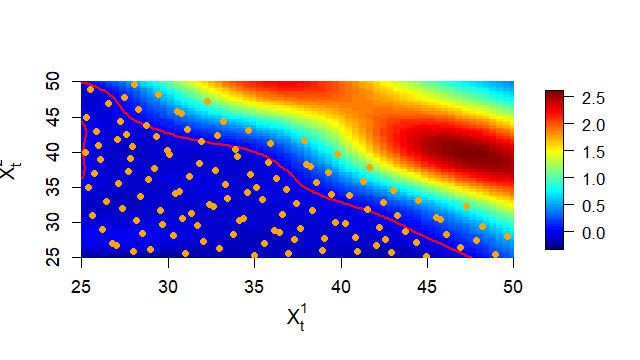
\includegraphics{figures/Same-with-GP-1.png} The above plot visualizes
the stopping boundary (red contour) and the fitted timing value (the
stopping region is the level set where the timing value is negative). We
also display the underlying Sobol QMC design of size 150.

To do a proper comparison between the fits we create a single
out-of-sample database and run both stopping rules on it.

\begin{Shaded}
\begin{Highlighting}[]
\NormalTok{NN <-}\StringTok{ }\DecValTok{16000}
\NormalTok{MM <-}\StringTok{ }\DecValTok{25}
\KeywordTok{set.seed}\NormalTok{(}\DecValTok{101}\NormalTok{)}
\NormalTok{mygr <-}\StringTok{ }\KeywordTok{list}\NormalTok{()}
\NormalTok{mygr[[}\DecValTok{1}\NormalTok{]] <-}\StringTok{ }\NormalTok{model2d}\OperatorTok{$}\KeywordTok{sim.func}\NormalTok{( }\KeywordTok{matrix}\NormalTok{(}\KeywordTok{rep}\NormalTok{(model2d}\OperatorTok{$}\NormalTok{x0, NN), }\DataTypeTok{nrow=}\NormalTok{NN, }\DataTypeTok{byrow=}\NormalTok{T), model2d, model2d}\OperatorTok{$}\NormalTok{dt)}
\ControlFlowTok{for}\NormalTok{ (i }\ControlFlowTok{in} \DecValTok{2}\OperatorTok{:}\NormalTok{(MM}\OperatorTok{+}\DecValTok{1}\NormalTok{))}
\NormalTok{   mygr[[i]] <-}\StringTok{ }\NormalTok{model2d}\OperatorTok{$}\KeywordTok{sim.func}\NormalTok{( mygr[[i}\OperatorTok{-}\DecValTok{1}\NormalTok{]], model2d, model2d}\OperatorTok{$}\NormalTok{dt)}
\CommentTok{# sanity check: European option value}
\KeywordTok{print}\NormalTok{(}\KeywordTok{mean}\NormalTok{( }\KeywordTok{exp}\NormalTok{(}\OperatorTok{-}\NormalTok{model2d}\OperatorTok{$}\NormalTok{r}\OperatorTok{*}\NormalTok{model2d}\OperatorTok{$}\NormalTok{T)}\OperatorTok{*}\KeywordTok{option.payoff}\NormalTok{(}\DataTypeTok{K=}\DecValTok{40}\NormalTok{,mygr[[MM]])))}
\end{Highlighting}
\end{Shaded}

\begin{verbatim}
## [1] 1.224074
\end{verbatim}

\begin{Shaded}
\begin{Highlighting}[]
\NormalTok{oos.lm <-}\StringTok{ }\KeywordTok{forward.sim.policy}\NormalTok{( mygr, MM, prob.lm}\OperatorTok{$}\NormalTok{fit, model2d)}
\NormalTok{oos.km <-}\StringTok{ }\KeywordTok{forward.sim.policy}\NormalTok{( mygr, MM, sob.km}\OperatorTok{$}\NormalTok{fit,  model2d)}
\KeywordTok{print}\NormalTok{( }\KeywordTok{c}\NormalTok{(}\KeywordTok{mean}\NormalTok{(oos.lm}\OperatorTok{$}\NormalTok{payoff), }\KeywordTok{mean}\NormalTok{(oos.km}\OperatorTok{$}\NormalTok{payoff)) )}
\end{Highlighting}
\end{Shaded}

\begin{verbatim}
## [1] 1.426594 1.431723
\end{verbatim}

\begin{Shaded}
\begin{Highlighting}[]
\KeywordTok{plot}\NormalTok{(oos.lm}\OperatorTok{$}\NormalTok{payoff, oos.km}\OperatorTok{$}\NormalTok{payoff)}
\end{Highlighting}
\end{Shaded}

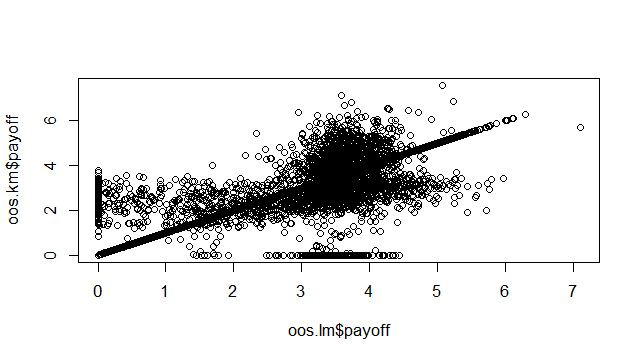
\includegraphics{figures/unnamed-chunk-2-1.png}

\subsection{Different types of regression
emulators}\label{different-types-of-regression-emulators}

The first function is \textbf{osp.prob.design}. This is classical RMC
that builds a design using a forward simulation of state trajectories.
Its main input is the \emph{method} which can take a large range of
regression methods. Specifics of each regression are controlled through
specifying \emph{required} respective model parameters.

First we consider a 1D example with \textbf{smooth.spline}. Note the
syntax: we use a total of 30000 trajectories, of which the first 10000
are reserved for testing, and the last 20000 is the training set. We
then also run a \textbf{randomForest}.

\begin{Shaded}
\begin{Highlighting}[]
\NormalTok{put1d.model}\OperatorTok{$}\NormalTok{nk=}\DecValTok{20}  \CommentTok{# number of knots for the smoothing spline}
\NormalTok{spl.eml.1dput <-}\StringTok{ }\KeywordTok{osp.prob.design}\NormalTok{(}\DecValTok{30000}\NormalTok{,put1d.model,}\DataTypeTok{subset=}\DecValTok{1}\OperatorTok{:}\DecValTok{10000}\NormalTok{,}\DataTypeTok{method=}\StringTok{"spline"}\NormalTok{)}
\end{Highlighting}
\end{Shaded}

\begin{verbatim}
## [1] "in-sample v_0 2.307815; and out-of-sample: 2.326382"
\end{verbatim}

\begin{Shaded}
\begin{Highlighting}[]
\NormalTok{put1d.model}\OperatorTok{$}\NormalTok{rf.ntree =}\StringTok{ }\DecValTok{200}  \CommentTok{# random forest parameters}
\NormalTok{put1d.model}\OperatorTok{$}\NormalTok{rf.maxnode=}\DecValTok{100}
\NormalTok{rf.eml.1dput <-}\StringTok{ }\KeywordTok{osp.prob.design}\NormalTok{(}\DecValTok{30000}\NormalTok{,put1d.model,}\DataTypeTok{subset=}\DecValTok{1}\OperatorTok{:}\DecValTok{10000}\NormalTok{,}\DataTypeTok{method=}\StringTok{"randomforest"}\NormalTok{)}
\end{Highlighting}
\end{Shaded}

\begin{verbatim}
## [1] "in-sample v_0 2.442872; and out-of-sample: 2.270105"
\end{verbatim}

As a a last example, We try \textbf{MARS} (multivariate adaptive
regression splines) from the \textbf{earth} package. We set the degree
to be 2, so that bases consist of linear/quadratic hinge functions.

\begin{Shaded}
\begin{Highlighting}[]
\NormalTok{put1d.model}\OperatorTok{$}\NormalTok{earth.deg =}\StringTok{ }\DecValTok{2}\NormalTok{;  }\CommentTok{# earth parameters}
\NormalTok{put1d.model}\OperatorTok{$}\NormalTok{earth.nk =}\StringTok{ }\DecValTok{100}\NormalTok{;}
\NormalTok{put1d.model}\OperatorTok{$}\NormalTok{earth.thresh =}\StringTok{ }\FloatTok{1e-8}
\NormalTok{mars.eml.1dput <-}\StringTok{ }\KeywordTok{osp.prob.design}\NormalTok{(}\DecValTok{30000}\NormalTok{,put1d.model,}\DataTypeTok{subset=}\DecValTok{1}\OperatorTok{:}\DecValTok{10000}\NormalTok{,}\DataTypeTok{method=}\StringTok{"earth"}\NormalTok{)}
\end{Highlighting}
\end{Shaded}

\begin{verbatim}
## [1] "in-sample v_0 2.301745; and out-of-sample: 2.229798"
\end{verbatim}

\subsection{Space-filling Batched
designs}\label{space-filling-batched-designs}

The second function, which is the workhorse of seqOSP, is
\textbf{osp.fixed.design}. It has three key parameters: input.domain
which controls the construction of the design, km.batch that controls
the replication amount and type which controls the regression method.
Because the design is now user-specified, its size can vary
step-by-step. The package also allows to vary the replication amounts.

We proceed to an overview of different ways to build a space-filling
design. The main issue is how to generate the bounding hyper-rectangle
that defines the effective input space. The package provides several
ways to do so.

The first example utilizes a user-defined simulation design that is used
as-is. The constructed ``sob150'' macro-design places 150 design sites
in a trianglular input domain, using a Sobol QMC sequence. For the
latter we employ the \emph{sobol} function in the \textbf{randtoolbox}
package. Based on model parameters, the input domain is the lower-left
triangle of \([25,55]^2\). Every site is then batched with 100
replications/site for a total simulation budget of \(N=15000\).

The \textbf{plt.2d.surf} function provides a way to visualize the
emulator of \(q(t,\cdot)\) at a single time-step, showing both the
timing value \(T(t,\cdot)\) and the stopping boundary (which is the
zero-contour of the latter). It also shows the respective design
\({\cal D}_t\) (the 150 points).

\begin{Shaded}
\begin{Highlighting}[]
\NormalTok{sob150 <-}\StringTok{ }\KeywordTok{sobol}\NormalTok{(}\DecValTok{276}\NormalTok{, }\DataTypeTok{d=}\DecValTok{2}\NormalTok{)}
\NormalTok{sob150 <-}\StringTok{ }\NormalTok{sob150[ }\KeywordTok{which}\NormalTok{( sob150[,}\DecValTok{1}\NormalTok{] }\OperatorTok{+}\StringTok{ }\NormalTok{sob150[,}\DecValTok{2}\NormalTok{] }\OperatorTok{<=}\StringTok{ }\DecValTok{1}\NormalTok{) ,]  }\CommentTok{# a lot are on the diagonal}
\NormalTok{sob150 <-}\StringTok{ }\DecValTok{25}\OperatorTok{+}\DecValTok{30}\OperatorTok{*}\NormalTok{sob150}

\NormalTok{model2d}\OperatorTok{$}\NormalTok{km.batch <-}\StringTok{ }\DecValTok{100}
\NormalTok{model2d}\OperatorTok{$}\NormalTok{pilot.nsims =}\StringTok{ }\DecValTok{0}
\NormalTok{model2d}\OperatorTok{$}\NormalTok{covfamily=}\StringTok{"matern5_2"}
\NormalTok{model2d}\OperatorTok{$}\NormalTok{N =}\StringTok{ }\DecValTok{500}   \CommentTok{# size of unique design sites; effective size is smaller as only in-the-money sites are kept}

\NormalTok{put2d.sobol.km <-}\StringTok{ }\KeywordTok{osp.fixed.design}\NormalTok{(model2d,}\DataTypeTok{input.dom=}\NormalTok{sob150, }\DataTypeTok{method=}\StringTok{"km"}\NormalTok{)}
\KeywordTok{plt.2d.surf}\NormalTok{(put2d.sobol.km}\OperatorTok{$}\NormalTok{fit[[}\DecValTok{12}\NormalTok{]], }\DataTypeTok{x=}\KeywordTok{seq}\NormalTok{(}\DecValTok{24}\NormalTok{,}\DecValTok{52}\NormalTok{,}\DataTypeTok{len=}\DecValTok{101}\NormalTok{),}\DataTypeTok{y=}\KeywordTok{seq}\NormalTok{(}\DecValTok{24}\NormalTok{,}\DecValTok{52}\NormalTok{,}\DataTypeTok{len=}\DecValTok{101}\NormalTok{),}\DataTypeTok{ub=}\DecValTok{10}\NormalTok{)}
\end{Highlighting}
\end{Shaded}

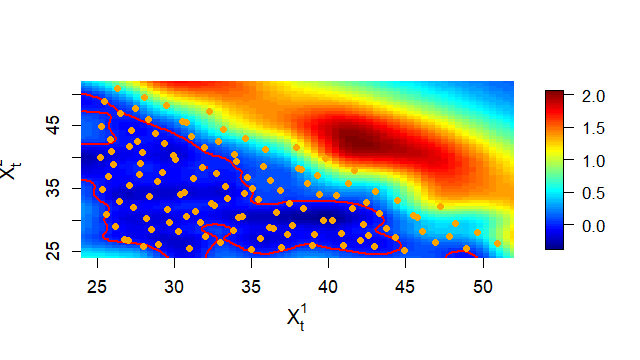
\includegraphics{figures/Sobol-pre-specified-1.png}

Secondly, we use an adaptive LHS design using some pilot simulations of
\(X_{0:T}\). Here \emph{input.dom=0.02} makes the LHS space-fill a box
between the 2nd and 98th percentiles of the pilot.nsim=1000 pilot
trajectories at each time step. The pilot trajectories act as
``scaffolding,'' organically expanding the input domain as \(t\) grows.

\begin{Shaded}
\begin{Highlighting}[]
\NormalTok{model2d}\OperatorTok{$}\NormalTok{pilot.nsims <-}\StringTok{ }\DecValTok{1000}
\NormalTok{model2d}\OperatorTok{$}\NormalTok{N =}\StringTok{ }\DecValTok{500}   \CommentTok{# size of unique design sites; effective size is smaller as only in-the-money sites are kept}
\NormalTok{model2d}\OperatorTok{$}\NormalTok{qmc.method <-}\StringTok{ }\OtherTok{NULL}
\NormalTok{put2d.lhsAdaptive.km <-}\StringTok{ }\KeywordTok{osp.fixed.design}\NormalTok{(model2d,}\DataTypeTok{input.dom=}\FloatTok{0.02}\NormalTok{, }\DataTypeTok{method=}\StringTok{"km"}\NormalTok{)}
\KeywordTok{par}\NormalTok{(}\DataTypeTok{mfrow=}\KeywordTok{c}\NormalTok{(}\DecValTok{1}\NormalTok{,}\DecValTok{2}\NormalTok{))}
\KeywordTok{plt.2d.surf}\NormalTok{(put2d.lhsAdaptive.km}\OperatorTok{$}\NormalTok{fit[[}\DecValTok{10}\NormalTok{]],}\DataTypeTok{x=}\KeywordTok{seq}\NormalTok{(}\DecValTok{24}\NormalTok{,}\DecValTok{52}\NormalTok{,}\DataTypeTok{len=}\DecValTok{101}\NormalTok{),}\DataTypeTok{y=}\KeywordTok{seq}\NormalTok{(}\DecValTok{24}\NormalTok{,}\DecValTok{52}\NormalTok{,}\DataTypeTok{len=}\DecValTok{101}\NormalTok{))}
\KeywordTok{plt.2d.surf}\NormalTok{(put2d.lhsAdaptive.km}\OperatorTok{$}\NormalTok{fit[[}\DecValTok{20}\NormalTok{]],}\DataTypeTok{x=}\KeywordTok{seq}\NormalTok{(}\DecValTok{24}\NormalTok{,}\DecValTok{52}\NormalTok{,}\DataTypeTok{len=}\DecValTok{101}\NormalTok{),}\DataTypeTok{y=}\KeywordTok{seq}\NormalTok{(}\DecValTok{24}\NormalTok{,}\DecValTok{52}\NormalTok{,}\DataTypeTok{len=}\DecValTok{101}\NormalTok{))}
\end{Highlighting}
\end{Shaded}

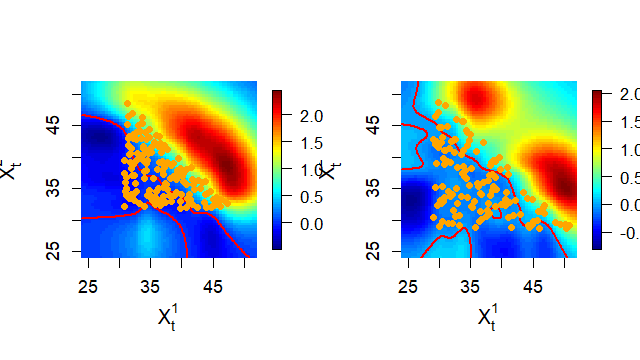
\includegraphics{figures/LHS-quantile-design-1.png}

If we set \emph{input.dom=-1} then the full range of the pilot scenarios
is used. Here we space-fill using a Halton QMC sequence. In addition, we
also train the \textbf{DiceKriging} model hyperparameters, which is the
Stochastic Kriging metamodel. Here for variety sake we pick a Gaussian
kernel.

\begin{Shaded}
\begin{Highlighting}[]
\NormalTok{model2d}\OperatorTok{$}\NormalTok{pilot.nsims <-}\StringTok{ }\DecValTok{1000}
\NormalTok{model2d}\OperatorTok{$}\NormalTok{km.upper <-}\StringTok{ }\DecValTok{20}
\NormalTok{model2d}\OperatorTok{$}\NormalTok{N =}\StringTok{ }\DecValTok{500}   \CommentTok{# size of unique design sites; effective size is smaller as only in-the-money sites are kept}
\NormalTok{model2d}\OperatorTok{$}\NormalTok{qmc.method <-}\StringTok{ }\NormalTok{randtoolbox}\OperatorTok{::}\NormalTok{halton}
\NormalTok{model2d}\OperatorTok{$}\NormalTok{covfamily <-}\StringTok{ "gauss"}
\NormalTok{put2d.haltonRange.trainkm <-}\StringTok{ }\KeywordTok{osp.fixed.design}\NormalTok{(model2d,}\DataTypeTok{input.dom=}\OperatorTok{-}\DecValTok{1}\NormalTok{, }\DataTypeTok{method=}\StringTok{"trainkm"}\NormalTok{)}
\KeywordTok{par}\NormalTok{(}\DataTypeTok{mfrow=}\KeywordTok{c}\NormalTok{(}\DecValTok{1}\NormalTok{,}\DecValTok{2}\NormalTok{))}
\KeywordTok{plt.2d.surf}\NormalTok{(put2d.haltonRange.trainkm}\OperatorTok{$}\NormalTok{fit[[}\DecValTok{10}\NormalTok{]],}\DataTypeTok{x=}\KeywordTok{seq}\NormalTok{(}\DecValTok{26}\NormalTok{,}\DecValTok{48}\NormalTok{,}\DataTypeTok{len=}\DecValTok{101}\NormalTok{),}\DataTypeTok{y=}\KeywordTok{seq}\NormalTok{(}\DecValTok{26}\NormalTok{,}\DecValTok{48}\NormalTok{,}\DataTypeTok{len=}\DecValTok{101}\NormalTok{))}
\KeywordTok{plt.2d.surf}\NormalTok{(put2d.haltonRange.trainkm}\OperatorTok{$}\NormalTok{fit[[}\DecValTok{20}\NormalTok{]],}\DataTypeTok{x=}\KeywordTok{seq}\NormalTok{(}\DecValTok{26}\NormalTok{,}\DecValTok{48}\NormalTok{,}\DataTypeTok{len=}\DecValTok{101}\NormalTok{),}\DataTypeTok{y=}\KeywordTok{seq}\NormalTok{(}\DecValTok{26}\NormalTok{,}\DecValTok{48}\NormalTok{,}\DataTypeTok{len=}\DecValTok{101}\NormalTok{))}
\end{Highlighting}
\end{Shaded}

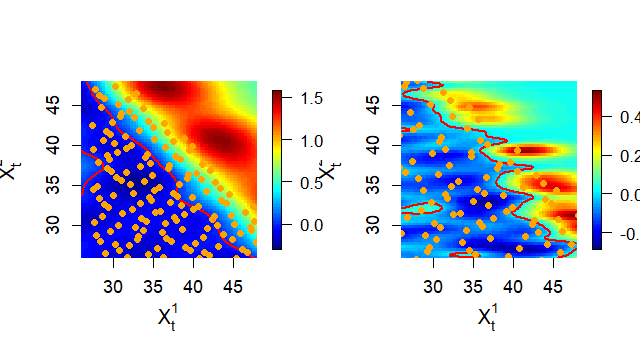
\includegraphics{figures/Halton-probabilistic-design-1.png}

\begin{Shaded}
\begin{Highlighting}[]
\KeywordTok{coef}\NormalTok{(put2d.haltonRange.trainkm}\OperatorTok{$}\NormalTok{fit[[}\DecValTok{15}\NormalTok{]])}
\end{Highlighting}
\end{Shaded}

\begin{verbatim}
## $trend
## [1] 0.1625656
##
## $range
## [1] 3.605977 1.163375
##
## $shape
## numeric(0)
##
## $sd2
## [1] 0.073349
##
## $nugget
## numeric(0)
\end{verbatim}

\subsubsection{Heteroskedastic GP
emulator}\label{heteroskedastic-gp-emulator}

The classical GP emulator assumes homoskedastic Gaussian simulation
noise. To tackle the strong heteroskedasticity encountered in our
context, we have utilized above the Stochastic Kriging (SK) approach. SK
utilizes a replicated design to locally estimate
\(\sigma^2(x) = \mathbb{Var}(\epsilon(x))\). This estimation is done
empirically via the classical MC variance estimator based on the batch
of \(r\) pathwise rewards starting at the same \(x\):
\[ \hat{\sigma^2(x)} = \frac{1}{r-1} \sum_{i=1}^r (y^i - \bar{y})^2.\]
To be reliable, this strategy necessitates using large batch sizes \(r\)
(called \textbf{n.reps} in mlOSP); in practice we find that \(r \gg 20\)
is necessary. For example, in the previous example we used
\(n.reps = 100\).

An alternative framework directly aims to learn \(\sigma^2(\cdot)\) via
a second spatial model that is jointly inferred with the standard mean
response. This has been recently implemented (Binois et al 2018) in the
\textbf{hetGP} package that we now illustrate. The main advantage of
using \textbf{hetGP} is the ability to lower the replication counts

\begin{Shaded}
\begin{Highlighting}[]
\NormalTok{model2d}\OperatorTok{$}\NormalTok{pilot.nsims <-}\StringTok{ }\DecValTok{1000}
\NormalTok{model2d}\OperatorTok{$}\NormalTok{km.upper <-}\StringTok{ }\DecValTok{20}
\NormalTok{model2d}\OperatorTok{$}\NormalTok{km.batch <-}\StringTok{ }\DecValTok{25}
\NormalTok{model2d}\OperatorTok{$}\NormalTok{covfamily <-}\StringTok{ "Matern5_2"}  \CommentTok{# note that hetGP has a slightly different naming convention for kernels}
\NormalTok{model2d}\OperatorTok{$}\NormalTok{N =}\StringTok{ }\DecValTok{1000}   \CommentTok{# size of unique design sites; effective size is smaller as only in-the-money sites are kept}
\NormalTok{model2d}\OperatorTok{$}\NormalTok{qmc.method <-}\StringTok{ }\NormalTok{randtoolbox}\OperatorTok{::}\NormalTok{halton}
\NormalTok{put2d.haltonAdaptive.hetgp <-}\StringTok{ }\KeywordTok{osp.fixed.design}\NormalTok{(model2d,}\DataTypeTok{input.dom=}\FloatTok{0.02}\NormalTok{, }\DataTypeTok{method=}\StringTok{"hetgp"}\NormalTok{)}
\end{Highlighting}
\end{Shaded}

\begin{verbatim}
## Homoskedastic model has higher log-likelihood:  -8930.404  compared to  -8942.43
## Return homoskedastic model
## Homoskedastic model has higher log-likelihood:  -9597.036  compared to  -9611.793
## Return homoskedastic model
## Homoskedastic model has higher log-likelihood:  -10319.91  compared to  -10331.29
## Return homoskedastic model
## Homoskedastic model has higher log-likelihood:  -11183.22  compared to  -11210.02
## Return homoskedastic model
## Homoskedastic model has higher log-likelihood:  -17780.54  compared to  -17784.91
## Return homoskedastic model
## Homoskedastic model has higher log-likelihood:  -18557.02  compared to  -18564.43
## Return homoskedastic model
## Homoskedastic model has higher log-likelihood:  -21844.39  compared to  -21850.73
## Return homoskedastic model
## Homoskedastic model has higher log-likelihood:  -21265.29  compared to  -21271.86
## Return homoskedastic model
## Homoskedastic model has higher log-likelihood:  -22178.58  compared to  -22190.17
## Return homoskedastic model
\end{verbatim}

\begin{Shaded}
\begin{Highlighting}[]
\KeywordTok{par}\NormalTok{(}\DataTypeTok{mfrow=}\KeywordTok{c}\NormalTok{(}\DecValTok{1}\NormalTok{,}\DecValTok{3}\NormalTok{))}
\KeywordTok{plt.2d.surf}\NormalTok{(put2d.haltonAdaptive.hetgp}\OperatorTok{$}\NormalTok{fit[[}\DecValTok{6}\NormalTok{]],}\DataTypeTok{x=}\KeywordTok{seq}\NormalTok{(}\DecValTok{26}\NormalTok{,}\DecValTok{48}\NormalTok{,}\DataTypeTok{len=}\DecValTok{101}\NormalTok{),}\DataTypeTok{y=}\KeywordTok{seq}\NormalTok{(}\DecValTok{26}\NormalTok{,}\DecValTok{48}\NormalTok{,}\DataTypeTok{len=}\DecValTok{101}\NormalTok{))}
\KeywordTok{plt.2d.surf}\NormalTok{(put2d.haltonAdaptive.hetgp}\OperatorTok{$}\NormalTok{fit[[}\DecValTok{14}\NormalTok{]],}\DataTypeTok{x=}\KeywordTok{seq}\NormalTok{(}\DecValTok{26}\NormalTok{,}\DecValTok{48}\NormalTok{,}\DataTypeTok{len=}\DecValTok{101}\NormalTok{),}\DataTypeTok{y=}\KeywordTok{seq}\NormalTok{(}\DecValTok{26}\NormalTok{,}\DecValTok{48}\NormalTok{,}\DataTypeTok{len=}\DecValTok{101}\NormalTok{))}
\KeywordTok{plt.2d.surf}\NormalTok{(put2d.haltonAdaptive.hetgp}\OperatorTok{$}\NormalTok{fit[[}\DecValTok{22}\NormalTok{]],}\DataTypeTok{x=}\KeywordTok{seq}\NormalTok{(}\DecValTok{26}\NormalTok{,}\DecValTok{48}\NormalTok{,}\DataTypeTok{len=}\DecValTok{101}\NormalTok{),}\DataTypeTok{y=}\KeywordTok{seq}\NormalTok{(}\DecValTok{26}\NormalTok{,}\DecValTok{48}\NormalTok{,}\DataTypeTok{len=}\DecValTok{101}\NormalTok{))}
\end{Highlighting}
\end{Shaded}

\begin{center}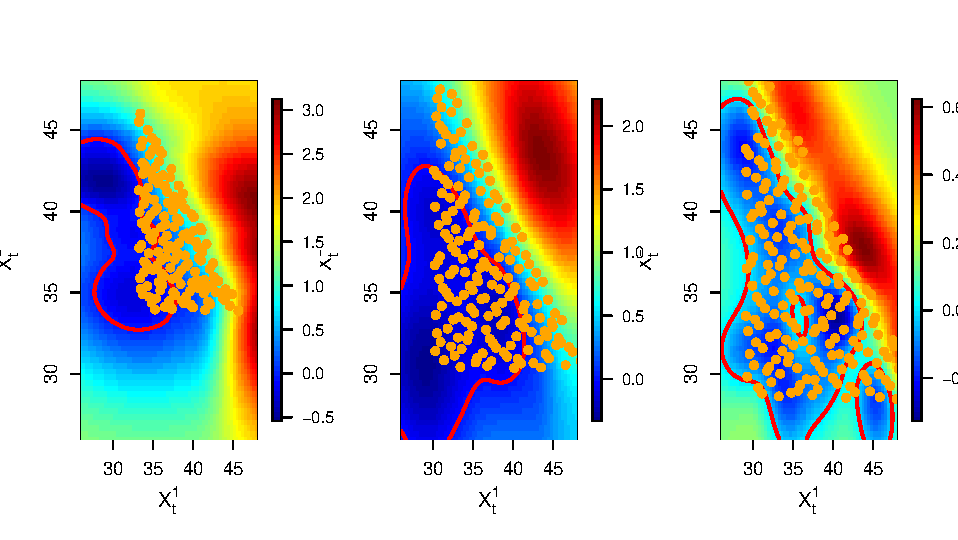
\includegraphics{figures/hetGP-2D-1} \end{center}

\begin{Shaded}
\begin{Highlighting}[]
\KeywordTok{summary}\NormalTok{(put2d.haltonAdaptive.hetgp}\OperatorTok{$}\NormalTok{fit[[}\DecValTok{14}\NormalTok{]])}
\end{Highlighting}
\end{Shaded}

\begin{verbatim}
## N =  7625  n =  305  d =  2
## Matern5_2  covariance lengthscale values of the main process:  8.281551 4.587073
## Variance/scale hyperparameter:  4.005986
## Summary of Lambda values:
##    Min. 1st Qu.  Median    Mean 3rd Qu.    Max.
##  0.2720  

\end{verbatim}

\begin{Shaded}
\begin{Highlighting}[]
\KeywordTok{plt.2d.surf}\NormalTok{(put2d.mcu.tp}\OperatorTok{$}\NormalTok{fit[[}\DecValTok{10}\NormalTok{]],}\DataTypeTok{x=}\KeywordTok{seq}\NormalTok{(}\DecValTok{26}\NormalTok{,}\DecValTok{48}\NormalTok{,}\DataTypeTok{len=}\DecValTok{101}\NormalTok{),}\DataTypeTok{y=}\KeywordTok{seq}\NormalTok{(}\DecValTok{26}\NormalTok{,}\DecValTok{48}\NormalTok{,}\DataTypeTok{len=}\DecValTok{101}\NormalTok{),}
            \DataTypeTok{sub=}\KeywordTok{sprintf}\NormalTok{(}\StringTok{"%4f"}\NormalTok{,}\KeywordTok{mean}\NormalTok{(oos.mcu.tp}\OperatorTok{$}\NormalTok{payoff)))}
\end{Highlighting}
\end{Shaded}

\begin{verbatim}
## Warning in (object$nu + object$psi - 2)/(object$nu + n1 - 2) * as.vector(object$sigma2 - : Recycling array of length 1 in array-vector arithmetic is deprecated.
##   Use c() or as.vector() instead.
\end{verbatim}

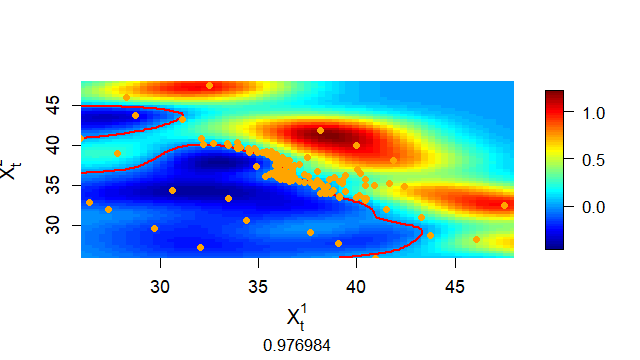
\includegraphics{figures/sequential-homtp-1.png}

\subsubsection{1D Put Example}\label{d-put-example}

We revisit the 1D Put example. Start with a grid of size 16 and go up to
100 total, or \(N=1000\) simulations.

\begin{Shaded}
\begin{Highlighting}[]
\KeywordTok{require}\NormalTok{(laGP)  }\CommentTok{# needed for distance function }
\NormalTok{model.seq1d <-}\StringTok{ }\NormalTok{put1d.model}

\NormalTok{option.payoff <-}\StringTok{ }\NormalTok{put.payoff}
\NormalTok{model.seq1d}\OperatorTok{$}\NormalTok{adaptive.grid.loop <-}\StringTok{ }\DecValTok{100}  \CommentTok{# final design size }
\NormalTok{model.seq1d}\OperatorTok{$}\NormalTok{km.batch <-}\StringTok{ }\DecValTok{10}
\NormalTok{model.seq1d}\OperatorTok{$}\NormalTok{init.size <-}\StringTok{ }\DecValTok{16}  \CommentTok{# initial design size}
\NormalTok{model.seq1d}\OperatorTok{$}\NormalTok{init.grid <-}\StringTok{ }\KeywordTok{as.matrix}\NormalTok{(}\KeywordTok{seq}\NormalTok{(}\DecValTok{25}\NormalTok{,}\DecValTok{40}\NormalTok{,}\DataTypeTok{length=}\DecValTok{16}\NormalTok{))}
\NormalTok{model.seq1d}\OperatorTok{$}\NormalTok{lhs.rect <-}\StringTok{ }\KeywordTok{matrix}\NormalTok{(}\KeywordTok{c}\NormalTok{(}\DecValTok{25}\NormalTok{,}\DecValTok{40}\NormalTok{),}\DataTypeTok{ncol=}\DecValTok{2}\NormalTok{)}
\NormalTok{model.seq1d}\OperatorTok{$}\NormalTok{al.heuristic <-}\StringTok{ "csur"}
\NormalTok{model.seq1d}\OperatorTok{$}\NormalTok{covfamily <-}\StringTok{ "Matern5_2"}
\NormalTok{model.seq1d}\OperatorTok{$}\NormalTok{km.upper <-}\StringTok{ }\DecValTok{8}
\NormalTok{put1d.sur.hetgp <-}\StringTok{ }\KeywordTok{osp.seq.design}\NormalTok{(model.seq1d, }\DataTypeTok{method=}\StringTok{"hetgp"}\NormalTok{)}
\end{Highlighting}
\end{Shaded}



\begin{Shaded}
\begin{Highlighting}[]
\CommentTok{# out-of-sample evaluation}
\NormalTok{NN <-}\StringTok{ }\DecValTok{40000}
\NormalTok{MM <-}\StringTok{ }\DecValTok{25}
\KeywordTok{set.seed}\NormalTok{(}\DecValTok{102}\NormalTok{)}
\NormalTok{test.1d <-}\StringTok{ }\KeywordTok{list}\NormalTok{()}
\NormalTok{test.1d[[}\DecValTok{1}\NormalTok{]] <-}\StringTok{ }\NormalTok{model1}\OperatorTok{$}\KeywordTok{sim.func}\NormalTok{( }\KeywordTok{matrix}\NormalTok{(}\KeywordTok{rep}\NormalTok{(}\KeywordTok{c}\NormalTok{(}\DecValTok{40}\NormalTok{), NN), }\DataTypeTok{nrow=}\NormalTok{NN, }\DataTypeTok{byrow=}\NormalTok{T), model1, model1}\OperatorTok{$}\NormalTok{dt)}
\ControlFlowTok{for}\NormalTok{ (i }\ControlFlowTok{in} \DecValTok{2}\OperatorTok{:}\NormalTok{(MM}\OperatorTok{+}\DecValTok{1}\NormalTok{))}
\NormalTok{   test.1d[[i]] <-}\StringTok{ }\NormalTok{model1}\OperatorTok{$}\KeywordTok{sim.func}\NormalTok{( test.1d[[i}\OperatorTok{-}\DecValTok{1}\NormalTok{]], model1, model1}\OperatorTok{$}\NormalTok{dt)}
\NormalTok{oos.hetgp.1d <-}\StringTok{ }\KeywordTok{forward.sim.policy}\NormalTok{( test.1d, MM, put1d.sur.hetgp}\OperatorTok{$}\NormalTok{fit, model.seq1d)}
\KeywordTok{print}\NormalTok{(}\KeywordTok{mean}\NormalTok{(oos.hetgp.1d}\OperatorTok{$}\NormalTok{payoff))}
\end{Highlighting}
\end{Shaded}

\begin{verbatim}
## [1] 2.26985
\end{verbatim}

\begin{Shaded}
\begin{Highlighting}[]
\NormalTok{check.x <-}\StringTok{ }\KeywordTok{matrix}\NormalTok{(}\KeywordTok{seq}\NormalTok{(}\DecValTok{24}\NormalTok{, }\DecValTok{40}\NormalTok{, }\DataTypeTok{len=}\DecValTok{500}\NormalTok{))   }\CommentTok{# predictive sites}
\NormalTok{sur.pred <-}\StringTok{ }\KeywordTok{predict}\NormalTok{(put1d.sur.hetgp}\OperatorTok{$}\NormalTok{fit[[}\DecValTok{15}\NormalTok{]],}\DataTypeTok{x=}\NormalTok{check.x)  }\CommentTok{# at t=0.6}
\KeywordTok{plot}\NormalTok{(check.x, sur.pred}\OperatorTok{$}\NormalTok{mean, }\DataTypeTok{lwd=}\DecValTok{2}\NormalTok{, }\DataTypeTok{type=}\StringTok{"l"}\NormalTok{, }\DataTypeTok{xlim=}\KeywordTok{c}\NormalTok{(}\DecValTok{25}\NormalTok{,}\DecValTok{40}\NormalTok{), }\DataTypeTok{ylim=}\KeywordTok{c}\NormalTok{(}\OperatorTok{-}\FloatTok{0.4}\NormalTok{,}\FloatTok{1.1}\NormalTok{), }\DataTypeTok{xlab=}\StringTok{'X'}\NormalTok{, }\DataTypeTok{ylab=}\StringTok{'Timing Value'}\NormalTok{)}
\KeywordTok{lines}\NormalTok{(check.x, sur.pred}\OperatorTok{$}\NormalTok{mean}\OperatorTok{+}\DecValTok{2}\OperatorTok{*}\KeywordTok{sqrt}\NormalTok{(sur.pred}\OperatorTok{$}\NormalTok{sd2), }\DataTypeTok{lty=}\DecValTok{2}\NormalTok{,}\DataTypeTok{col=}\StringTok{"grey"}\NormalTok{)  }\CommentTok{# 95% CI band}
\KeywordTok{lines}\NormalTok{(check.x, sur.pred}\OperatorTok{$}\NormalTok{mean}\OperatorTok{-}\DecValTok{2}\OperatorTok{*}\KeywordTok{sqrt}\NormalTok{(sur.pred}\OperatorTok{$}\NormalTok{sd2), }\DataTypeTok{lty=}\DecValTok{2}\NormalTok{,}\DataTypeTok{col=}\StringTok{"grey"}\NormalTok{)}
\KeywordTok{abline}\NormalTok{(}\DataTypeTok{h=}\DecValTok{0}\NormalTok{,}\DataTypeTok{lty=}\DecValTok{2}\NormalTok{)}
\KeywordTok{rug}\NormalTok{(put1d.sur.hetgp}\OperatorTok{$}\NormalTok{fit[[}\DecValTok{15}\NormalTok{]]}\OperatorTok{$}\NormalTok{X0, }\DataTypeTok{quiet=}\OtherTok{TRUE}\NormalTok{)}
\KeywordTok{rug}\NormalTok{(model.seq1d}\OperatorTok{$}\NormalTok{init.grid, }\DataTypeTok{quiet=}\OtherTok{TRUE}\NormalTok{, }\DataTypeTok{col=}\StringTok{"red"}\NormalTok{,}\DataTypeTok{ticksize=}\FloatTok{0.05}\NormalTok{)}
\end{Highlighting}
\end{Shaded}

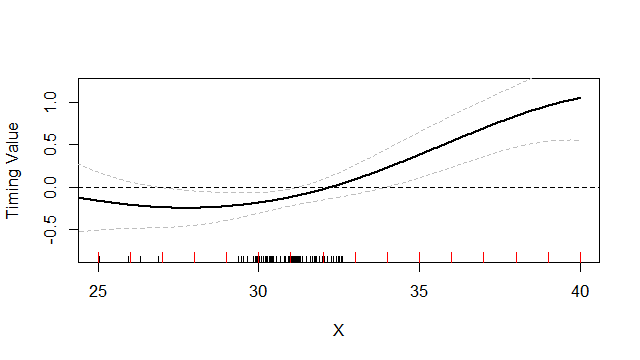
\includegraphics{figures/1dput-sequential-1.png}

\subsection{Building a New Model}\label{building-a-new-model}

As an example of how the user may easily work with \textbf{mlOSP}, we
proceed to show the step-by-step process of implementing a new example
based on the recent article by Cheridito et al (arxiv.org/1804.05394
(Becker, Cheridito, and Jentzen 2018)).

Specifically we consider a multivariate GBM model with asymmetric
volatilities and constant correlation. The payoff functional is of the
max-Call type already described above. We have \[ \label{eq:multi-gbm}
S^i_t = s^i_0 exp( [r-\delta_i-\sigma_i^2/2]t + \sigma_i W_t^i), \qquad i=1,\ldots, d
\] where the instantaneous correlation between \(W^i\) and \(W^j\) is
\(\rho_{ij}\). In the asymmetric example of Becker et al,
\(d=5, s^i_0 = s_0, \delta_i = \delta, \rho_{ij} = \rho\) and
\(\sigma_i = 0.08 i\) with other parameter values
\(\delta = 10\%, r = 5\%, \rho = 0\) and contract specification
\(s_0 = 90, T=3, K=100, M=9\).

We first define a new simulation function using the \emph{rmvnorm}
function in the \textbf{mvtnorm} library. To avoid passing too many
parameters, we introduce new \emph{model} fields \emph{rho} (taken to be
a constant) and \emph{sigma} (a vector of length d).

\begin{Shaded}
\begin{Highlighting}[]
\KeywordTok{require}\NormalTok{(mvtnorm)}
\end{Highlighting}
\end{Shaded}

\begin{verbatim}
## Loading required package: mvtnorm
\end{verbatim}

\begin{verbatim}
## Warning: package 'mvtnorm' was built under R version 3.4.3
\end{verbatim}

\begin{Shaded}
\begin{Highlighting}[]
\NormalTok{sim.corGBM <-}\StringTok{ }\ControlFlowTok{function}\NormalTok{( x0, model, dt)}
\NormalTok{\{}
\NormalTok{    sigm <-}\StringTok{ }\KeywordTok{kronecker}\NormalTok{(model}\OperatorTok{$}\NormalTok{sigma, }\KeywordTok{t}\NormalTok{(model}\OperatorTok{$}\NormalTok{sigma))  }\CommentTok{# matrix of sigma_i*sigma_j}
\NormalTok{    sigm <-}\StringTok{ }\NormalTok{model}\OperatorTok{$}\NormalTok{rho}\OperatorTok{*}\NormalTok{sigm }\OperatorTok{+}\StringTok{ }\NormalTok{(}\DecValTok{1}\OperatorTok{-}\NormalTok{model}\OperatorTok{$}\NormalTok{rho)}\OperatorTok{*}\KeywordTok{diag}\NormalTok{(model}\OperatorTok{$}\NormalTok{sigma}\OperatorTok{^}\DecValTok{2}\NormalTok{)  }\CommentTok{# correct the diagonal to be sigma_i^2}

    \CommentTok{# implement the correlated GBM, specify the covariance matrix and the mean, both are linear in 'dt'}
\NormalTok{    newX <-}\StringTok{ }\NormalTok{x0}\OperatorTok{*}\KeywordTok{exp}\NormalTok{( }\KeywordTok{rmvnorm}\NormalTok{(}\KeywordTok{nrow}\NormalTok{(x0), }\DataTypeTok{sig=}\NormalTok{sigm}\OperatorTok{*}\NormalTok{dt, }\DataTypeTok{mean=}\NormalTok{ (model}\OperatorTok{$}\NormalTok{r}\OperatorTok{-}\StringTok{ }\NormalTok{model}\OperatorTok{$}\NormalTok{div}\OperatorTok{-}\StringTok{ }\NormalTok{model}\OperatorTok{$}\NormalTok{sigma}\OperatorTok{^}\DecValTok{2}\OperatorTok{/}\DecValTok{2}\NormalTok{)}\OperatorTok{*}\NormalTok{dt) )}

    \KeywordTok{return}\NormalTok{ (newX)}
\NormalTok{\}}
\end{Highlighting}
\end{Shaded}

Next, we construct the problem instance, i.e.~the model in mlOSP
parlance.

\begin{Shaded}
\begin{Highlighting}[]
\NormalTok{modelBecker <-}\StringTok{ }\KeywordTok{list}\NormalTok{(}\DataTypeTok{dim=}\DecValTok{5}\NormalTok{,}\DataTypeTok{sigma=}\FloatTok{0.08}\OperatorTok{*}\NormalTok{(}\DecValTok{1}\OperatorTok{:}\DecValTok{5}\NormalTok{), }\DataTypeTok{r=} \FloatTok{0.05}\NormalTok{, }\DataTypeTok{div=}\FloatTok{0.1}\NormalTok{, }\DataTypeTok{rho=}\DecValTok{0}\NormalTok{, }\DataTypeTok{x0 =} \KeywordTok{rep}\NormalTok{(}\DecValTok{90}\NormalTok{,}\DecValTok{5}\NormalTok{), }\DataTypeTok{T=}\DecValTok{3}\NormalTok{, }\DataTypeTok{K=}\DecValTok{100}\NormalTok{, }\DataTypeTok{dt=}\DecValTok{1}\OperatorTok{/}\DecValTok{3}\NormalTok{, }
                    \DataTypeTok{sim.func=}\NormalTok{sim.corGBM, }\DataTypeTok{km.upper=}\KeywordTok{rep}\NormalTok{(}\DecValTok{100}\NormalTok{,}\DecValTok{5}\NormalTok{))}
\CommentTok{#model1 <- c(final.runs=0, K=40,x0=40,sigma=0.2,r=0.06,div=0,T=1,dt=0.04,dim=1,sim.func=sim.gbm,}
\CommentTok{# lhs.rect=c(25,40),init.size=15,km.cov=4,km.var=1,cand.len=1000,look.ahead=1)}
\end{Highlighting}
\end{Shaded}

For the design we consider a union of a space-filling design on
\([50,200]^d\) of size 400 and a probabilistic design of size 200. We
are now ready to test with a \emph{hetGP} metamodel which requires a few
more parameter specification

\begin{Shaded}
\begin{Highlighting}[]
\NormalTok{sf400 <-}\StringTok{ }\DecValTok{50} \OperatorTok{+}\StringTok{ }\DecValTok{150}\OperatorTok{*}\KeywordTok{sobol}\NormalTok{(}\DecValTok{400}\NormalTok{,}\DataTypeTok{d=}\DecValTok{5}\NormalTok{, }\DataTypeTok{scrambl=}\DecValTok{1}\NormalTok{)}
\NormalTok{pd200 <-}\StringTok{ }\KeywordTok{sim.corGBM}\NormalTok{( }\KeywordTok{matrix}\NormalTok{(}\KeywordTok{rep}\NormalTok{(modelBecker}\OperatorTok{$}\NormalTok{x0,}\DecValTok{200}\NormalTok{), }\DataTypeTok{nrow=}\DecValTok{200}\NormalTok{,}\DataTypeTok{byrow=}\NormalTok{T), modelBecker, modelBecker}\OperatorTok{$}\NormalTok{T)}
\NormalTok{option.payoff <-}\StringTok{ }\NormalTok{maxCall}
\NormalTok{modelBecker}\OperatorTok{$}\NormalTok{km.batch }\OperatorTok{<=}\StringTok{ }\DecValTok{50}
\end{Highlighting}
\end{Shaded}

\begin{verbatim}
## logical(0)
\end{verbatim}

\begin{Shaded}
\begin{Highlighting}[]
\NormalTok{modelBecker}\OperatorTok{$}\NormalTok{covtype <-}\StringTok{ "Matern5_2"}
\NormalTok{modelBecker}\OperatorTok{$}\NormalTok{pilot.nsims <-}\StringTok{ }\DecValTok{100}
\NormalTok{modelBecker}\OperatorTok{$}\NormalTok{N <-}\StringTok{ }\DecValTok{600}
\NormalTok{modelBecker}\OperatorTok{$}\NormalTok{look.ahead <-}\StringTok{ }\DecValTok{1}
\CommentTok{#  pilot.nsims=1000, look.ahead=1, N=100,km.batch=50,km.upper=c(20,20), cand.len=1000, covtype="Matern5_2" )}

\NormalTok{beckerFit <-}\StringTok{ }\KeywordTok{osp.fixed.design}\NormalTok{(modelBecker,}\DataTypeTok{input.dom=}\KeywordTok{rbind}\NormalTok{(sf400,pd200), }\DataTypeTok{method=}\StringTok{"hetgp"}\NormalTok{)}
\end{Highlighting}
\end{Shaded}

\begin{verbatim}
## Homoskedastic model has higher log-likelihood:  -2466.147  compared to  -2466.195
## Return homoskedastic model
## Homoskedastic model has higher log-likelihood:  -2606.585  compared to  -2606.607
## Return homoskedastic model
## Homoskedastic model has higher log-likelihood:  -2886.634  compared to  -2886.709
## Return homoskedastic model
\end{verbatim}

We finally test on an out-of-sample set of scenarios.

\begin{Shaded}
\begin{Highlighting}[]
\NormalTok{NN <-}\StringTok{ }\DecValTok{100000}
\NormalTok{MM <-}\StringTok{ }\DecValTok{9}
\KeywordTok{set.seed}\NormalTok{(}\DecValTok{102}\NormalTok{)}
\NormalTok{test.Becker <-}\StringTok{ }\KeywordTok{list}\NormalTok{()}
\NormalTok{test.Becker[[}\DecValTok{1}\NormalTok{]] <-}\StringTok{ }\NormalTok{modelBecker}\OperatorTok{$}\KeywordTok{sim.func}\NormalTok{( }\KeywordTok{matrix}\NormalTok{(}\KeywordTok{rep}\NormalTok{(modelBecker}\OperatorTok{$}\NormalTok{x0, NN), }\DataTypeTok{nrow=}\NormalTok{NN, }\DataTypeTok{byrow=}\NormalTok{T), }
\NormalTok{                                          modelBecker, modelBecker}\OperatorTok{$}\NormalTok{dt)}
\ControlFlowTok{for}\NormalTok{ (i }\ControlFlowTok{in} \DecValTok{2}\OperatorTok{:}\NormalTok{MM)}
\NormalTok{   test.Becker[[i]] <-}\StringTok{ }\NormalTok{modelBecker}\OperatorTok{$}\KeywordTok{sim.func}\NormalTok{( test.Becker[[i}\OperatorTok{-}\DecValTok{1}\NormalTok{]], modelBecker, modelBecker}\OperatorTok{$}\NormalTok{dt)}
\CommentTok{# sanity check: European option value}
\KeywordTok{print}\NormalTok{(}\KeywordTok{mean}\NormalTok{( }\KeywordTok{exp}\NormalTok{(}\OperatorTok{-}\NormalTok{modelBecker}\OperatorTok{$}\NormalTok{r}\OperatorTok{*}\NormalTok{modelBecker}\OperatorTok{$}\NormalTok{T)}\OperatorTok{*}\KeywordTok{option.payoff}\NormalTok{(}\DataTypeTok{K=}\DecValTok{100}\NormalTok{,test.Becker[[MM]])))}
\end{Highlighting}
\end{Shaded}

\begin{verbatim}
## [1] 24.5945
\end{verbatim}

\begin{Shaded}
\begin{Highlighting}[]
\NormalTok{oos <-}\StringTok{ }\KeywordTok{forward.sim.policy}\NormalTok{( test.Becker, MM, beckerFit}\OperatorTok{$}\NormalTok{fit, modelBecker)}\OperatorTok{$}\NormalTok{payoff}
\KeywordTok{print}\NormalTok{( }\KeywordTok{c}\NormalTok{(}\KeywordTok{mean}\NormalTok{(oos) }\OperatorTok{-}\StringTok{ }\FloatTok{1.96}\OperatorTok{*}\KeywordTok{sd}\NormalTok{(oos)}\OperatorTok{/}\KeywordTok{sqrt}\NormalTok{(NN), }\KeywordTok{mean}\NormalTok{(oos)}\OperatorTok{+}\FloatTok{1.96}\OperatorTok{*}\KeywordTok{sd}\NormalTok{(oos)}\OperatorTok{/}\KeywordTok{sqrt}\NormalTok{(NN)) )}
\end{Highlighting}
\end{Shaded}

\begin{verbatim}
## [1] 15.57871 15.88224
\end{verbatim}

Voila. This can be compared against the reported interval of {[}27.63,
27.69{]}. We note the very high standard deviation of realized payoffs
which leads to a wide credible interval of the final answer. Thus,
obtaining tight bounds requires a very large out-of-sample test set.

\hypertarget{refs}{}
\hypertarget{ref-Broadie}{}
Andersen, L., and M. Broadie. 2004. ``A Primal-Dual Simulation Algorithm
for Pricing Multi-Dimensional American Options.'' \emph{Management
Science} 50 (9): 1222--34.

\hypertarget{ref-CheriditoJentzen18}{}
Becker, Sebastian, Patrick Cheridito, and Arnulf Jentzen. 2018. ``Deep
Optimal Stopping.'' arXiv preprint arXiv:1804.05394.

\hypertarget{ref-BouchardWarin10}{}
Bouchard, B., and X. Warin. 2011. ``Monte-Carlo Valorisation of American
Options: Facts and New Algorithms to Improve Existing Methods.'' In
\emph{Numerical Methods in Finance}, edited by R. Carmona, P. Del Moral,
P. Hu, and N. Oudjane. Vol. 12. Springer Proceedings in Mathematics.
Springer.

\hypertarget{ref-GL13}{}
Gramacy, R.B., and M. Ludkovski. 2015. ``Sequential Design for Optimal
Stopping Problems.'' \emph{SIAM Journal on Financial Mathematics} 6 (1):
748--75. \url{http://arXiv.org/abs/1309.3832}.

\hypertarget{ref-Kohler12lasso}{}
Kohler, Michael, and Adam Krzyżak. 2012. ``Pricing of American Options
in Discrete Time Using Least Squares Estimates with Complexity
Penalties.'' \emph{Journal of Statistical Planning and Inference} 142
(8). Elsevier: 2289--2307.

\hypertarget{ref-LS}{}
Longstaff, F.A., and E.S. Schwartz. 2001. ``Valuing American Options by
Simulations: A Simple Least Squares Approach.'' \emph{The Review of
Financial Studies} 14: 113--48.


\end{document}
